\documentclass[12pt]{article}

%Paquetes a utilizarse
\usepackage[width=7in, height=9.5in, top=0.75in, papersize={8.5in,11in}]{geometry}
\usepackage[spanish]{babel} 
\decimalpoint
\usepackage[utf8]{inputenc}
\usepackage{bbding}
\usepackage[colorlinks = true, linkcolor = blue, urlcolor = BlueViolet, citecolor = OliveGreen]{hyperref}
\usepackage{graphicx}
\usepackage{amssymb,amsthm,amsmath}
\usepackage{enumerate}
\usepackage{array,multicol,multirow}
\usepackage{xcolor}
\usepackage{fancybox,tcolorbox}
\usepackage{caption,subcaption,float,tabularx}
\usepackage{enumitem}

\theoremstyle{definition}
\newtheorem{corolario}{Corolario}
\newtheorem{lema}[corolario]{Lema}
\newtheorem{proposicion}[corolario]{Proposición}
\newtheorem{teorema}[corolario]{Teorema}
\newtheorem{propiedad}[corolario]{Propiedad}
\newtheorem*{observacion}{Observación}
\newtheorem{definicion}{Definición}
\newtheorem*{demostracion}{Demostración}
\newtheorem{ejemplo}{Ejemplo}
\newtheorem{problema}{Problema}
\newtheorem*{solucion}{Solución}
\newtheorem{ejercicio}{\PencilRightDown \  Ejercicio}
\newtheorem{step}{Paso}
\newtheorem{credito}{Crédito}

\usepackage{tikz}
\usetikzlibrary{arrows.meta,babel,calc,positioning}

\renewcommand{\arraystretch}{1.5}
\providecommand{\abs}[1]{\lvert#1\rvert}
\providecommand{\norm}[1]{\lVert#1\rVert}

\renewcommand{\tabularxcolumn}[1]{m{#1}}
\newcommand{\Evaluacion}[4]{
\setcounter{ejercicio}{0}
\noindent\begin{tabular}{lcr}
	\includegraphics[height=3cm]{Logos/logo-UES.png}\hspace{2.5em}
	&
	\includegraphics[height=2.75cm]{Logos/logo-PJT.png}
	& 
	\hspace{2.5em}\includegraphics[height=2.75cm]{Logos/logo-MINEDUCYT.png}
\end{tabular}

\hfill

\begin{center}
    
    UNIVERSIDAD DE EL SALVADOR
    \\PROGRAMA JÓVENES TALENTO
    \\FDTC 2022
    \\#2
    \\Nivel Olímpico C de Matemáticas

\end{center}

\begin{center}
    #1
\end{center}

%\textbf{Nombre}: \enspace\hrulefill

#3

\input{#4}
\newpage
}

\newtheorem{obs}{Observación}

%\usepackage[margin=2.5cm]{geometry}
%\usepackage{wasysym}
%\usepackage{stmaryrd,textcomp}
%\usepackage{pgf,tikz}
%\usetikzlibrary{arrows}

\parskip = 2mm   %%%% genera un espacio de X mm entre lo párrafos
\parindent = 3mm
\usepackage{multicol}
\usepackage{iwona}

\newcommand{\tema}{Principios fundamentales}
\newcommand{\fecha}{Viernes, 2 de diciembre de 2022}
\newcommand{\sesion}{Corto 2}

\begin{document}
%\thispagestyle{empty}
%\newpage
\thispagestyle{empty}

\begin{figure}[h] 
	\begin{minipage}[b]{0.26\textwidth}
		\begin{center}
			
\includegraphics[height=3cm]{Logos/UES.png}
			\par\end{center}
	\end{minipage} 
	\begin{minipage}[b]{0.46\textwidth}
		\begin{center}
			UNIVERSIDAD DE EL SALVADOR\\ [0.1cm]
			PROGRAMA JÓVENES TALENTO\\ [0.1cm]
	        FDTC 2022\\ [0.1cm]
                NIVEL 5\\ [0.1cm]
			COMBINATORIA 
			\par\end{center}
	\end{minipage} 
	\begin{minipage}[b]{0.05\textwidth}
		\begin{center}
			
\includegraphics[height=2cm]{Logos/LOGO PJT.png}
			\par\end{center}
	\end{minipage}
\end{figure}

\begin{center}
    \begin{tabular}{p{4.5cm} p{7cm} p{4.5cm}}
        \tema & \centering\fecha & \hfill\sesion
    \end{tabular}
\end{center}

\begin{problema}
Determinar cuántos triángulos aparecen en la siguiente figura.
\begin{figure}[h!]
    \centering
    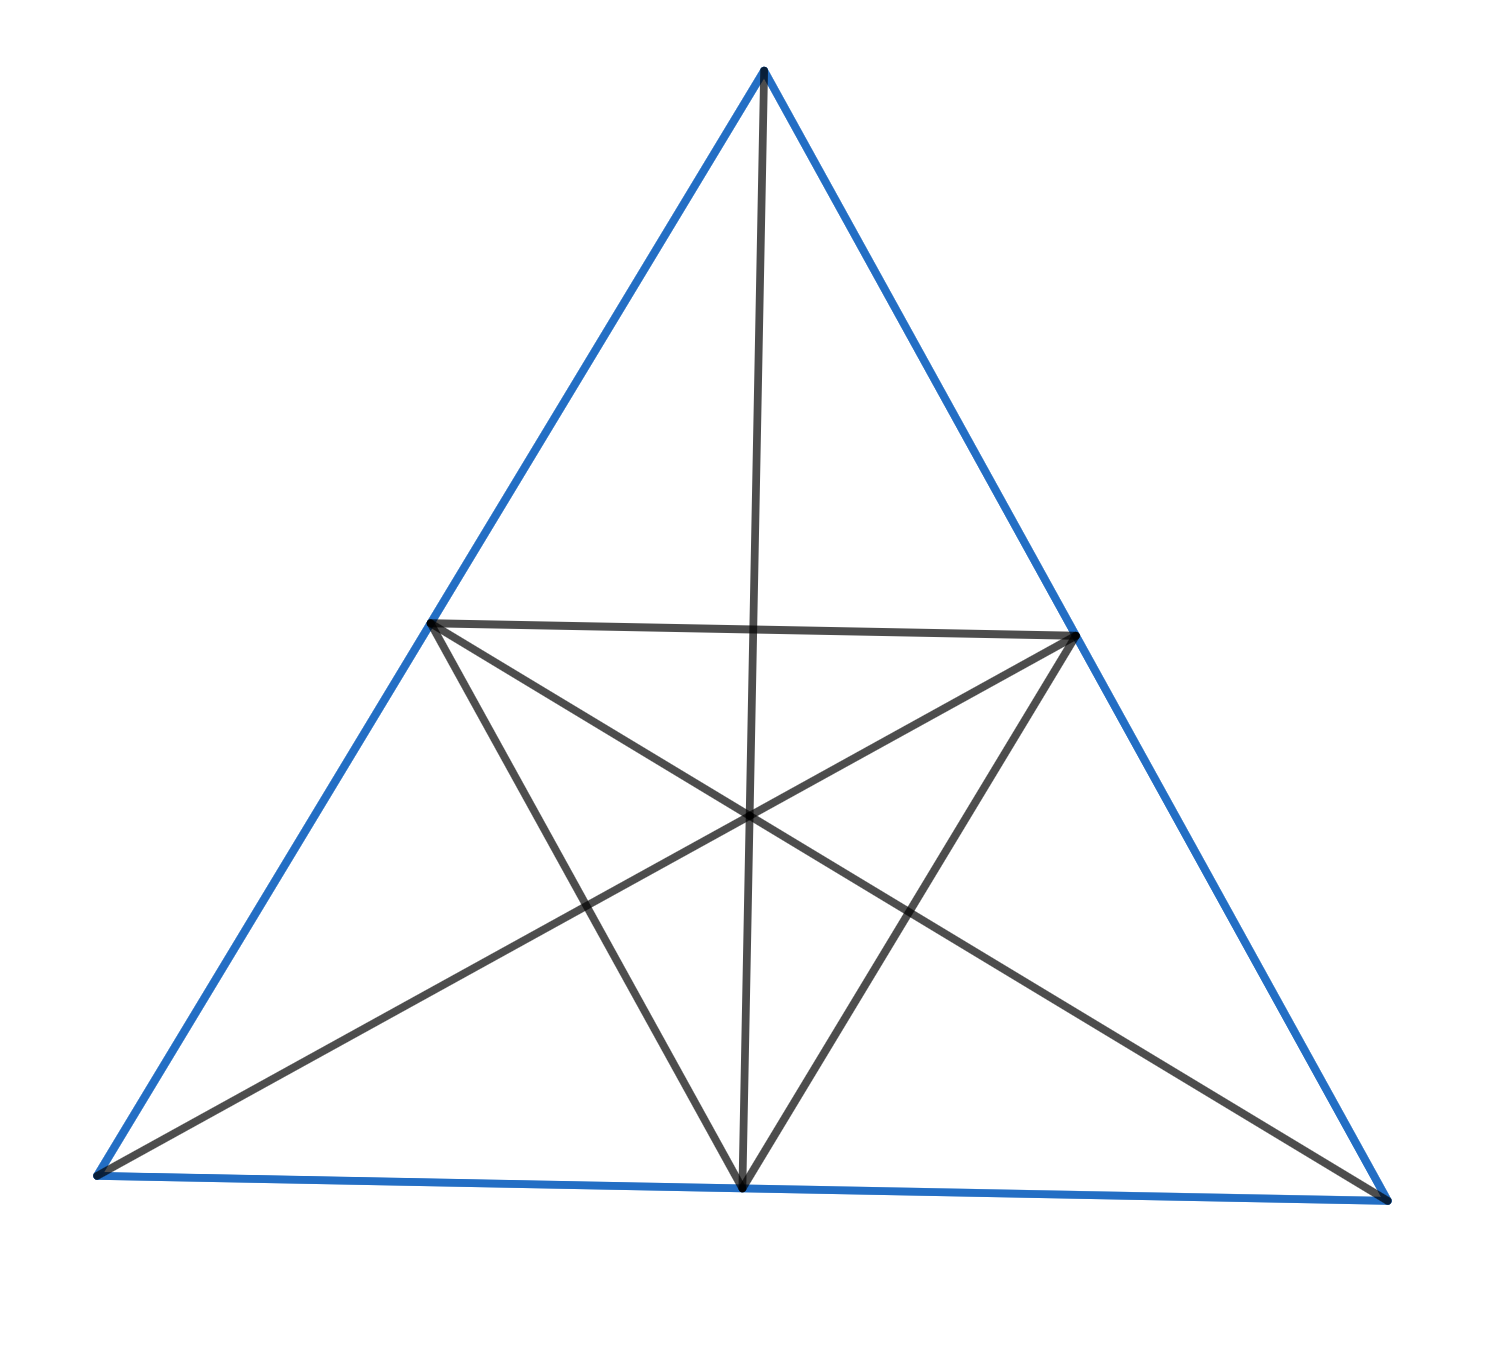
\includegraphics[scale=0.2]{Imagenes/IMG1/img_corto2.png}
    %\caption{}
    %\label{fig1}
\end{figure}
\end{problema}

\begin{problema}
Suponga un tablero generado por un cuadrado de $6\times 6$, es decir, de $36$ casillas. En eso vamos a ubicar dos torres (piezas de ajedrez) de tal manera que no se capturen entre ellas. ¿De cuántas maneras se podría realizar esto?

{\small \textbf{Hint.} \textit{La torre se mueve en una línea recta horizontal o vertical a lo largo de cualquier número de casillas desocupadas, hasta que alcanza el final del tablero o es bloqueado por otra pieza. No puede saltar sobre otras piezas. La torre captura de la misma manera en la que se mueve, ocupando la casilla en la que está la pieza oponente. La torre puede colocarse en cualquier casilla del tablero, por tanto es una de las piezas más poderosas.}}
\end{problema}

\textbf{Crédito extra:} En un concurso navideño, una persona debe adivinar un número decimal. El animador que está dirigiendo el concurso le da las siguientes pistas: \textit{el número tiene $3$ dígitos enteros y $2$ decimales; los dígitos pueden ser $1$, $2$, $3$, $7$ y $8$ y los decimales $6$ y $9$. Además el número es mayor que $300$}. ¿Cuántos números pudiéramos formar con las pistas que nos han dado, si se permite la repetición de los dígitos $1$ y $2$? 

\end{document}